\section{Evaluation Metrics} \label{eval}

Text-to-SQL tasks can be evaluated by two methods: accurate matching rate and execution accuracy rate. Predicted SQL statements are compared with standard statements to determine how accurate the match is.
By splitting the predicted SQL statement and definitive statement into multiple clauses according to keywords, we can solve the problem of matching errors caused by order of the where clause. The matching is successful as long as the elements in both sets are the same.

% pics/acc1.png
\begin{figure}[htb]
    \centering
    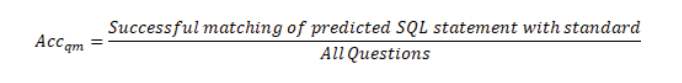
\includegraphics[width=0.6\textwidth]{pics/acc1.png}
    % \caption{Accurate matching rate}
    \label{fig:acc1}
\end{figure}

When using the correct predicted SQL statements, the correct execution rate refers to the proportion of questions that can receive the correct answers from the database.

% pics/acc2.png
\begin{figure}[htb]
    \centering
    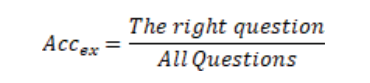
\includegraphics[width=0.4\textwidth]{pics/acc2.png}
    % \caption{Accuracy rate of the predicted SQL statements}
    \label{fig:acc2}
\end{figure}

By predicting the key F1 values for SQL statements, the model can also be evaluated.

% pics/f1.png
\begin{figure}[htb]
    \centering
    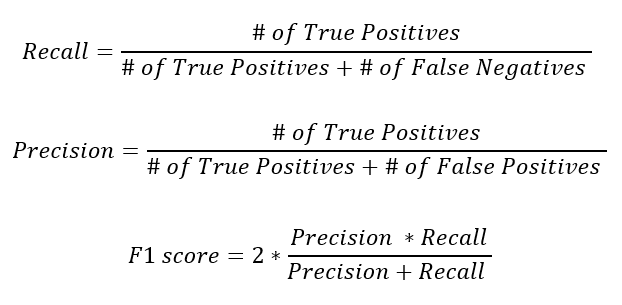
\includegraphics[width=0.6\textwidth]{pics/f1.png}
    % \caption{F1 score for SQL statements}
    \label{fig:f1}
\end{figure}

\subsection{Exact String Matching}
\subsection{ESM: Exact Set Matching}

the current Spider official metric

\subsection{Distilled Test Suites}
